\documentclass[a4paper,12pt]{article}

\usepackage[T2A]{fontenc} 
\usepackage[utf8]{inputenc}
\usepackage[english,russian]{babel}
\usepackage{listings}
\usepackage[dvips]{graphicx}
\usepackage{indentfirst}
\usepackage{color}
\usepackage{hyperref}
\usepackage{amsmath}
\usepackage{amssymb}
\usepackage{geometry}
\geometry{left=1.5cm}
\geometry{right=1.5cm}
\geometry{top=1cm}
\geometry{bottom=2cm}

\graphicspath{{images/}}

\begin{document}
\sloppy

\lstset{
	basicstyle=\small,
	stringstyle=\ttfamily,
	showstringspaces=false,
	columns=fixed,
	breaklines=true,
	numbers=right,
	numberstyle=\tiny
}

\newtheorem{Def}{Определение}[section]
\newtheorem{Th}{Теорема}
\newtheorem{Lem}[Th]{Лемма}
\newenvironment{Proof}
	{\par\noindent{\bf Доказательство.}}
	{\hfill$\scriptstyle\blacksquare$}
\newenvironment{Solution}
	{\par\noindent{\bf Решение.}}
	{\hfill$\scriptstyle\blacksquare$}


\begin{flushright}
	Кринкин М. Ю. группа 504 (SE)
\end{flushright}

\section{Домашнее задание 2}
\paragraph{Задание 1.} Сколько существует шестизначных чисел, сумма цифр которых четна? А если берутся все числа от 1 до 999999?
\begin{Solution}
Отбросим первую цифру числа, т. к. для нее нужны особые условия (она не может быть равна 0), таким образом переходим к рассмотрению всех чисел от 0 до 99999. Каждый разряд может быть четным или нечетным, если в разряде содержится четная цифра сопоставим ей 0, если в разряде стоит нечетная цифра, то 1. Тогда каждому числу соответствует битовый вектор длины 5, причем, если сумма цифр исходного числа четна, то и сумма единиц соответствующего вектора тоже четна. Число битовых векторов длины 5 с четным числом единиц равно $2^4$, в каждый такой вектор переходит $5^5$ чисел, тогда общее число чисел от 0 до 99999 с четной суммой цифр равно $5^52^4$ и аналогичное количество чисел с нечетной суммой. Теперь вернем  рассмотрение первый разряд, он может принимать значения из множества $\{1, 2, 3, 4, 5, 6, 7, 8, 9\}$. Дописав четный разряд $\{2, 4, 6, 8\}$ четность суммы цифр полученного числа не меняется, а дописав $\{1, 3, 5, 7, 9\}$ четность суммы цифр измениятся, в итоге получаем:
\[
	9 \cdot 5^5 \cdot 2^4
\]
Для всех чисел от 0 до 999999 можно провести аналогичное рассуждение, в итоге получаем: $5^6 \cdot 2^5$
\end{Solution}
\paragraph{Задание 2.} Сколько существует пятизначных четных чисел, в которых не одна цифра не повторяется?
\begin{Solution}
На последнем месте в этом числе могут стоять цифры $\{0, 2, 4, 6, 8\}$, а на первом месте могут стоять все цифры, кроме нуля $\{1, 2, 3, 4, 5, 6, 7, 8, 9\}$. Просуммируем по количеству пятизначных чисел оканчивающихся на 0, 2, 4, 6 и 8:
\[
	9 \cdot 8 \cdot 7 \cdot 6 + 8 \cdot 8 \cdot 7 \cdot 6 + 8 \cdot 8 \cdot 7 \cdot 6 + 8 \cdot 8 \cdot 7 \cdot 6 + 8 \cdot 8 \cdot 7 \cdot 6
\]
\end{Solution}
\paragraph{Задание 3.} Длина дороги из одного города (A) до другого города (B) равна 999 км. Вдоль дороги стоят километровые столбы, на которых написаны расстояния и от A, и до B: $0|999, 1|998, ... , 999|0$. Сколько среди этих столбов таких, на которых нанесены только 2 различные цифры?
\begin{Solution}
Очевидно, что эти различные цифры, обозначим их $x_1$ и $x_2$, в сумме должны давать 9, все такие пары легко перечислить ($\{0, 9\}, \{1, 8\}, \{2, 7\}, \{3, 6\}, \{4, 5\}$). Составим таблицу, которая поможет решить задачу:
\[
	\begin{matrix}
		x_1 & x_1 & x_1 && x_2 & x_2 & x_2 \\
		x_1 & x_1 & x_2 && x_2 & x_2 & x_1 \\
		x_1 & x_2 & x_1 && x_2 & x_1 & x_2 \\
		x_1 & x_2 & x_2 && x_2 & x_1 & x_1 \\
		x_2 & x_1 & x_1 && x_1 & x_2 & x_2 \\
		x_2 & x_1 & x_2 && x_1 & x_2 & x_1 \\
		x_2 & x_2 & x_1 && x_1 & x_1 & x_2 \\
		x_2 & x_2 & x_2 && x_1 & x_1 & x_1 \\
	\end{matrix}
\]
В левой и правой частях таблицы получатся расстояния до обоих городов, для записи которых используются только 2 цифры, например:
\[
	\begin{matrix}
		  &   & 0 & && 9 & 9 & 9 \\
		  &   & 9 & && 9 & 9 & 0 \\
		  & 9 & 0 & && 9 & 0 & 9 \\
		  & 9 & 9 & && 9 & 0 & 0 \\
		9 & 0 & 0 & &&   & 9 & 9 \\
		9 & 0 & 9 & &&   & 9 & 0 \\
		9 & 9 & 0 & &&   &   & 9 \\
		9 & 9 & 9 & &&   &   & 0 \\
	\end{matrix}
\]
Решение получается умножением количества строк таблицы на количество пар цифр, дающих с в сумме 9: $5 \cdot 8$
\end{Solution}
\paragraph{Задание 4.} Найти сумму всех трехзначных чисел, которые можно записать только с помощью цифр 1, 2, 3, 4. А если никакая цифра не должна повторяться дважды в записи числа?
\begin{Solution}
	Будем складывать поразрядно. Посчитаем количество чисел, в которых на i-ом месте (от 0 до 2) стоит цифра k $T = T_i^k = 4^2$ (если повторы допустимы) или $T = T_i^k = 3 \cdot 2$ (если повторы не допустимы), и как видно не зависит от разряда или цифры, сумма i-ого разряда всех чисел, удовлетворяющих условию, $10^i \sum_{k=1}^{4}k T_i^k = 10^i T \sum_{k=1}^{4} k = 10^i T 10 = 10^{i+1} T$, суммируя по всем трем разрядам получаем, для цифр с повторами:
\[
	1000 \cdot 16 + 100 \cdot 16 + 10 \cdot 16 = 16 \cdot 1110
\]
а для цифр без повторов:
\[
	1000 \cdot 6 + 100 \cdot 6 + 10 \cdot 6 = 6 \cdot 1110
\]
\end{Solution}
\paragraph{Задание 5. Старая} Имеются 15 различных сигнальных флагов и 3 различные мачты, на которых их вывешивают. Значение сигнала зависит от того, в каком порядке и на какой мачте вывешены флаги. Сколькими способами можно развесить эти флаги?
\begin{Solution}
Посмотрим на рисунок \ref{pic::ship}.
\begin{figure}[h]
	\noindent\center{
		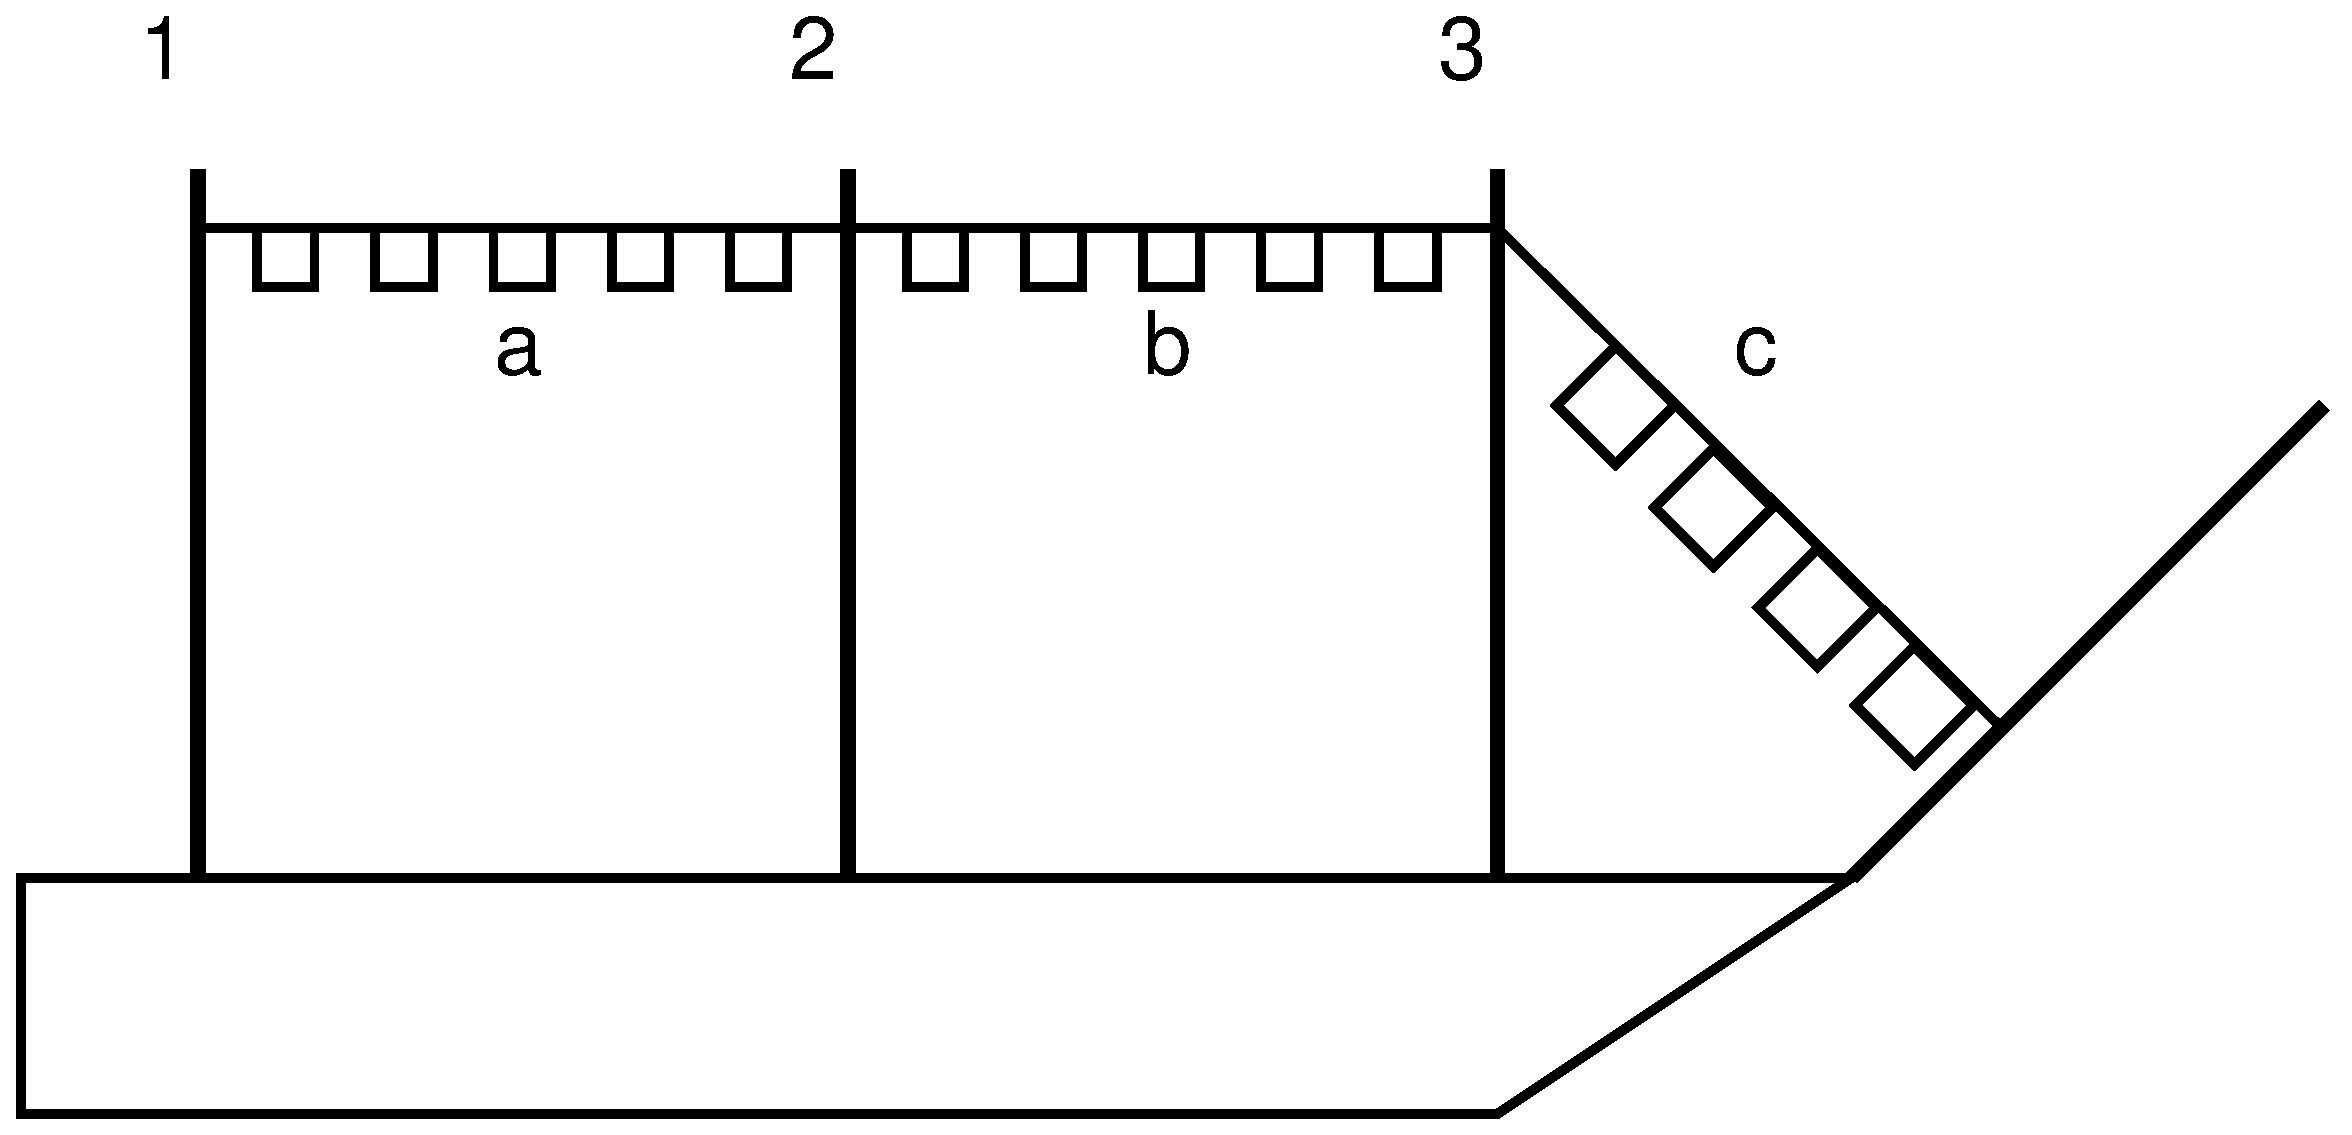
\includegraphics[width=0.3\linewidth]{ship.eps}
	}
	\caption{Кораблик}
	\label{pic::ship}
\end{figure}
Флаги висящие в пролете (a) - флаги первой мачты, в пролете (b) - флаги второй мачты, и (с) - флаги третьей. Таким образом, можно сказать, что задача сводится к распределению флагов по "контейнерам" - мачтам с учетом порядка флагов. Для подсчета добавим к флагам 2 неразличимых разделяющих предмета и посчитаем все возможные перестановки 17 различных предметов и поделим на все перестановки неразличимых разделяющих предметов: \[\frac{17!}{2!}\]
\end{Solution}
\paragraph{Задача 5. Новая} Сколько существует целых чисел между 0 и 1000, содержащих ровно одну цифру 7? А хотябы одну?
\begin{Solution}
Цифра 7 может стоять в первом (справа) разряде, во втором и в третьем, посчитаем количество чисел от 0 до 1000, в которых 7 стоит строго в одном разряде: $9 \cdot 9$ (т. е. фиксируем цифру 7 в одном разряде, в сотальных разрядах могут быть любые цифры кроме 7, включая и 0), тогда количество всех чисел содержащих ровно одну цифру 7 в записи равно: $3 \cdot 9 \cdot 9$, а количество чисел содержащих чотябы одну, можно вычислить посчитав общее количество 3-х значных чисел (1000 можно отбросит, и не опускать ведущие нули), т. е. $10^3 = 1000$, и вычесть числа не содержащие цифры 7, а таких $9^3 = 729$, в результате получаем: $1000 - 729 = 271$
\end{Solution}

\paragraph{Задание 6.} Доказать соотношение:
\[
	\begin{split}
		& P\left(n,k\right) = P\left(n-1,k\right)+k P\left(n-1,k-1\right)\\
		& P\left(n,0\right) = 1, \forall n \ge 0 \\
		& P\left(n,k\right) = 0, \forall k > n
	\end{split}
\]
\begin{Solution}
Комбинаторное доказательство. Как и в двух прошлых случаях, выделим один элемент из множества $X$ и разобьем все k-перестановки из n элементов, относительно выбранного элемента на два множества, первое ($\sum_{x \notin}$) содержит перстановки не содержащие выделенный элемент, а второе ($\sum_{x \in}$) содержит перестановки с этим элементом, причем выбранный элемент может стоять на любой из $k$ позиций. Мощности этих множеств:
\begin{itemize}
	\item $\left|\sum_{x \not\in}\right| = P\left(n-1,k\right)$

	\item $\left|\sum_{x \in}\right| = k \cdot P\left(n-1, k-1\right)$
\end{itemize}
\end{Solution}

\begin{Solution}
Доказательство, не комбинаторное.
\begin{multline*}
	\prod_{i=0}^{k-1}\left(n-i\right) = n \cdot \prod_{i=1}^{k-1} \left(n-i\right) = \\
	= n \cdot \prod_{i=0}^{k-2} \left(n-1-i\right) = \left(n-k+k\right) \cdot \prod_{i=0}^{k-2} = \\ 
	= \left(n-k\right) \cdot \prod_{i=0}^{k-2} \left(n-1-i\right)+k \cdot \prod_{i=0}^{k-2} \left(n-1-i\right) = \\ 
	= P\left(n-1,k\right) + k \cdot P \left(n-1, k-1\right)
\end{multline*}
\end{Solution}

\paragraph{Задача 7.} Пусть имеется уравнение $\sum_{i=1}^{n} a_i = k$. Необходимо узнать сколько целочисленных решений имеет это уравнение, при следующих ограничениях:
\begin{itemize}
\item $a_i \ge S_i$

\item $S = \sum_{i=1}^{n} S_i \le k$
\end{itemize}
\begin{Solution}
На каждую переменную наложено ограничение снизу, в этом случае мы делим $k$ единиц между $n$ позициями (переменными) с повторениями, а ограничение говорит только о том, что $S$ единиц уже распределены, таким образом осталось распределить $k-S$ единиц:
\[
	\left( \binom{n}{k-S} \right)
\]
\end{Solution}

\paragraph{Задача 8. } Пусть имеется уравнение $\sum_{i=1}^{n} a_i = k$. Необходимо узнать сколько целочисленных решений имеет это уравнение, при следующих ограничениях:
\begin{itemize}
\item $a_i \le m_i$

\item $m = \sum_{i=1}^{n} m_i \ge k$
\end{itemize}
\begin{Solution}
Пойдем путем наблюдений. Пусть $m=k$, то количество решений очевидно равно одному, далее рассмотрим случай $m=k+1$, в данном случае на всех переменных кроме одной будет выполняться условие $a_i = m_i$, а на одной $a_j + 1 = m_j$, т. е. мы выбираем среди n позиций одну. Далее рассмотрим $m=k+2$, по аналогии, выбираем среди n позиций 2, с повторениями и тд. Таким образом мы распределяем $m-k$ единиц "недобора" до границ $m_i$ с повторениями между $n$ границами:
\[
	\left(\binom{n}{m-k}\right)
\] 
\end{Solution}

\end{document}
